\documentclass[../main.tex]{subfiles}
\begin{document}
\subsubsection{Flickering as an alternative sign of critical thresholds}\label{subsubsec1.2.3}
Contemporary to the rise of indicators for CSD and their critics, another phenomenon was being observed to be a precursor of regime shifts. We mentioned above some indicators s.a. increase in variance and skewness to be prognostic of CSD albeit showing weaker signals w.r.t. autocorrelation \cite{Biggs09,Drake10,Carpenter11a}.
Changing skewness in the distribution of the realizations of the timeseries was first proposed in 2008 \cite{Guttal08} as an indicator of increasing asymmetry in a number of simulated ecosystems. 
In such paper the origin of a trend in skewness as the models approached a critical transition was linked to the asymmetric change of the potential landscape of the SDE.
This prescribes that the state of the system has particular directions, towards which it may tip to, that are more favourable than others.
This observation is considerably different from the flattening of the potential landscape that is found at the core of CSD and as such suggested that a novel precursor was being measured by the proposed EWS.
This new phenomenon (it was shown) did not rely on the linearisation of the dynamics around the stable equilibrium and instead considered the effects of high noise levels to be dominant close to the critical threshold where alternative attractors became \textit{``available"} to the system under large fluctuations.
It would be thus reasonable to expect that systems that do not feature such asymmetry in the presence of multi-stable states will not exhibit stronger signals than those that are instead purely associated to the flattening of the potential landscape as prescribed by CSD.
\paragraph{Mid 2010s}
In 2010 this intuition was further validated by approximating the shape of the potential function (and thus estimating the number of states available to the system at given parameter values) by polynomial fitting of the empirical distribution of timeseries data \cite{Livina10}. 
The method, termed potential analysis, succesfully detected an increased number of alternative stable states for ice-core proxy records of paleotemperature transitions at NGRIP, thus providing yet another indicator of asymetric changes in the potential landscape of a model. 
Similarly to the increase in skewness, also the increase in variance, previously linked to CSD, was discovered to occur in unsteady excursions of the state towards alternate basins of attraction. Brock and Carpenter \cite{Brock10} thus distinguished the two sources of increased variance in the already known CSD and the new phenomenon which they named flickering. 
\begin{figure}[H]
   \begin{subfigure}[b]{0.475\textwidth}
        \centering 
        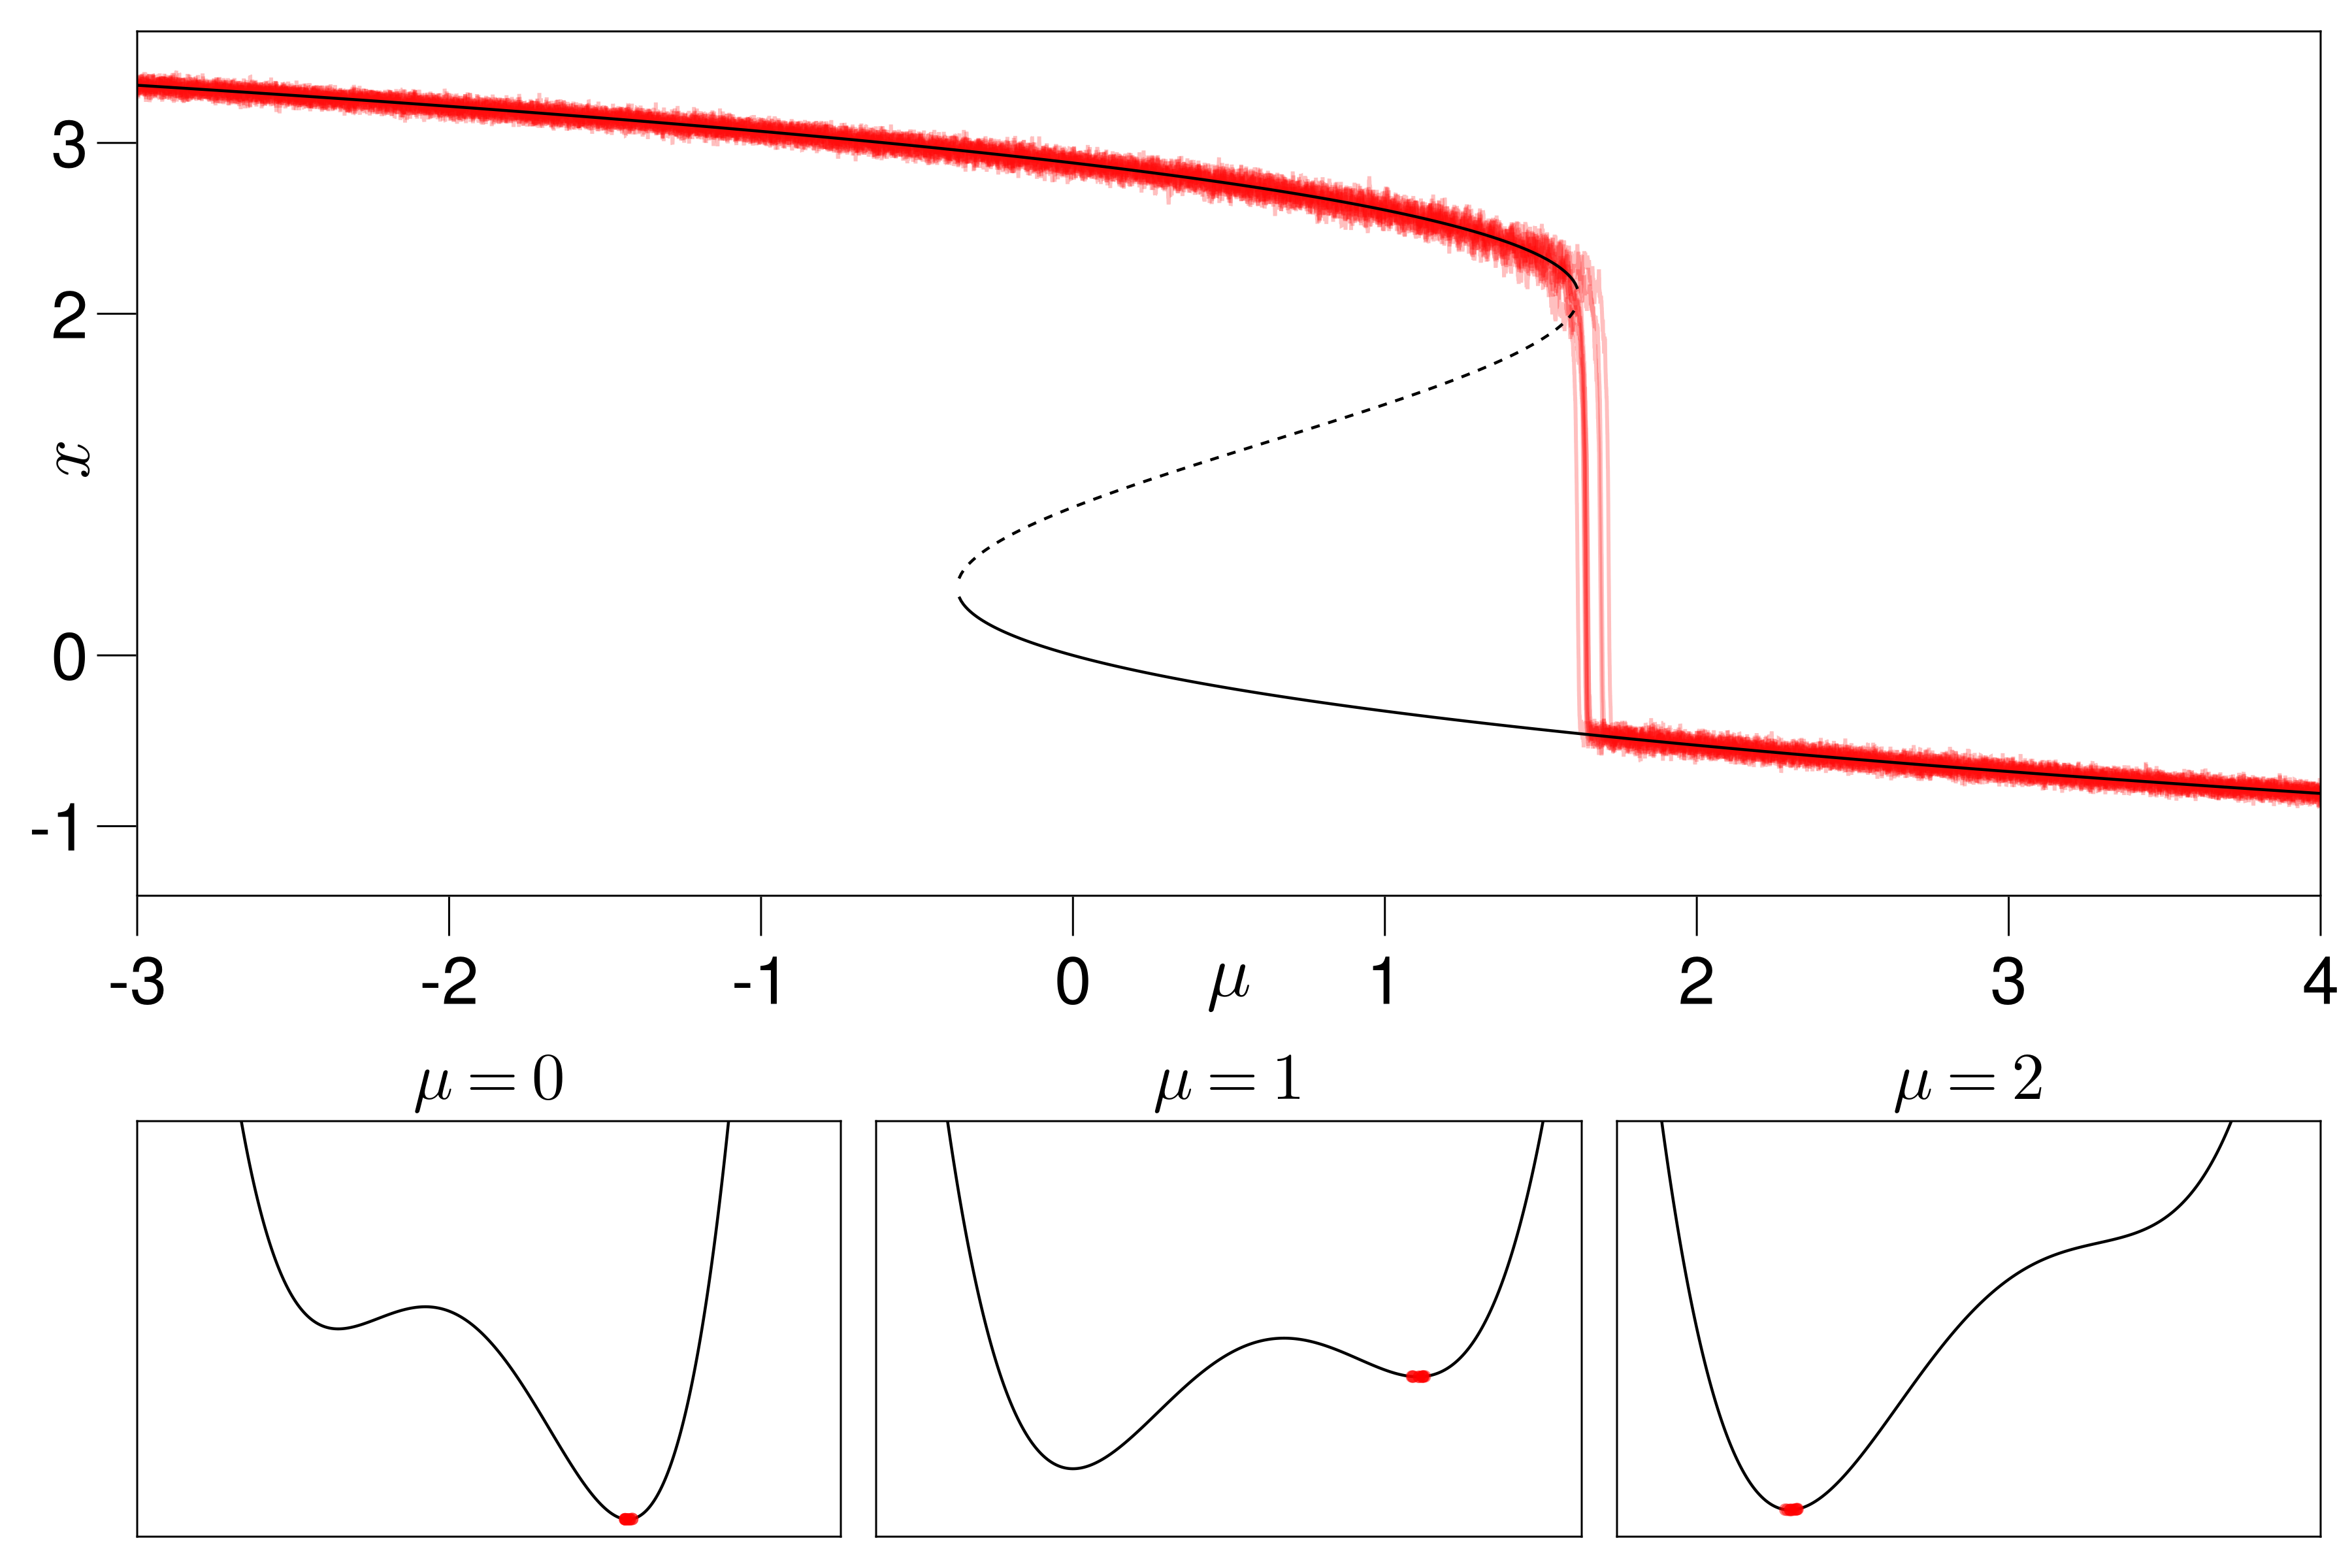
\includegraphics[keepaspectratio, width = \linewidth]{../figures/fig1.3.1.png}
        \caption{}
        \label{fig1.3.1}
   \end{subfigure}
   \hfill
   \begin{subfigure}[b]{0.475\textwidth}
        \centering 
        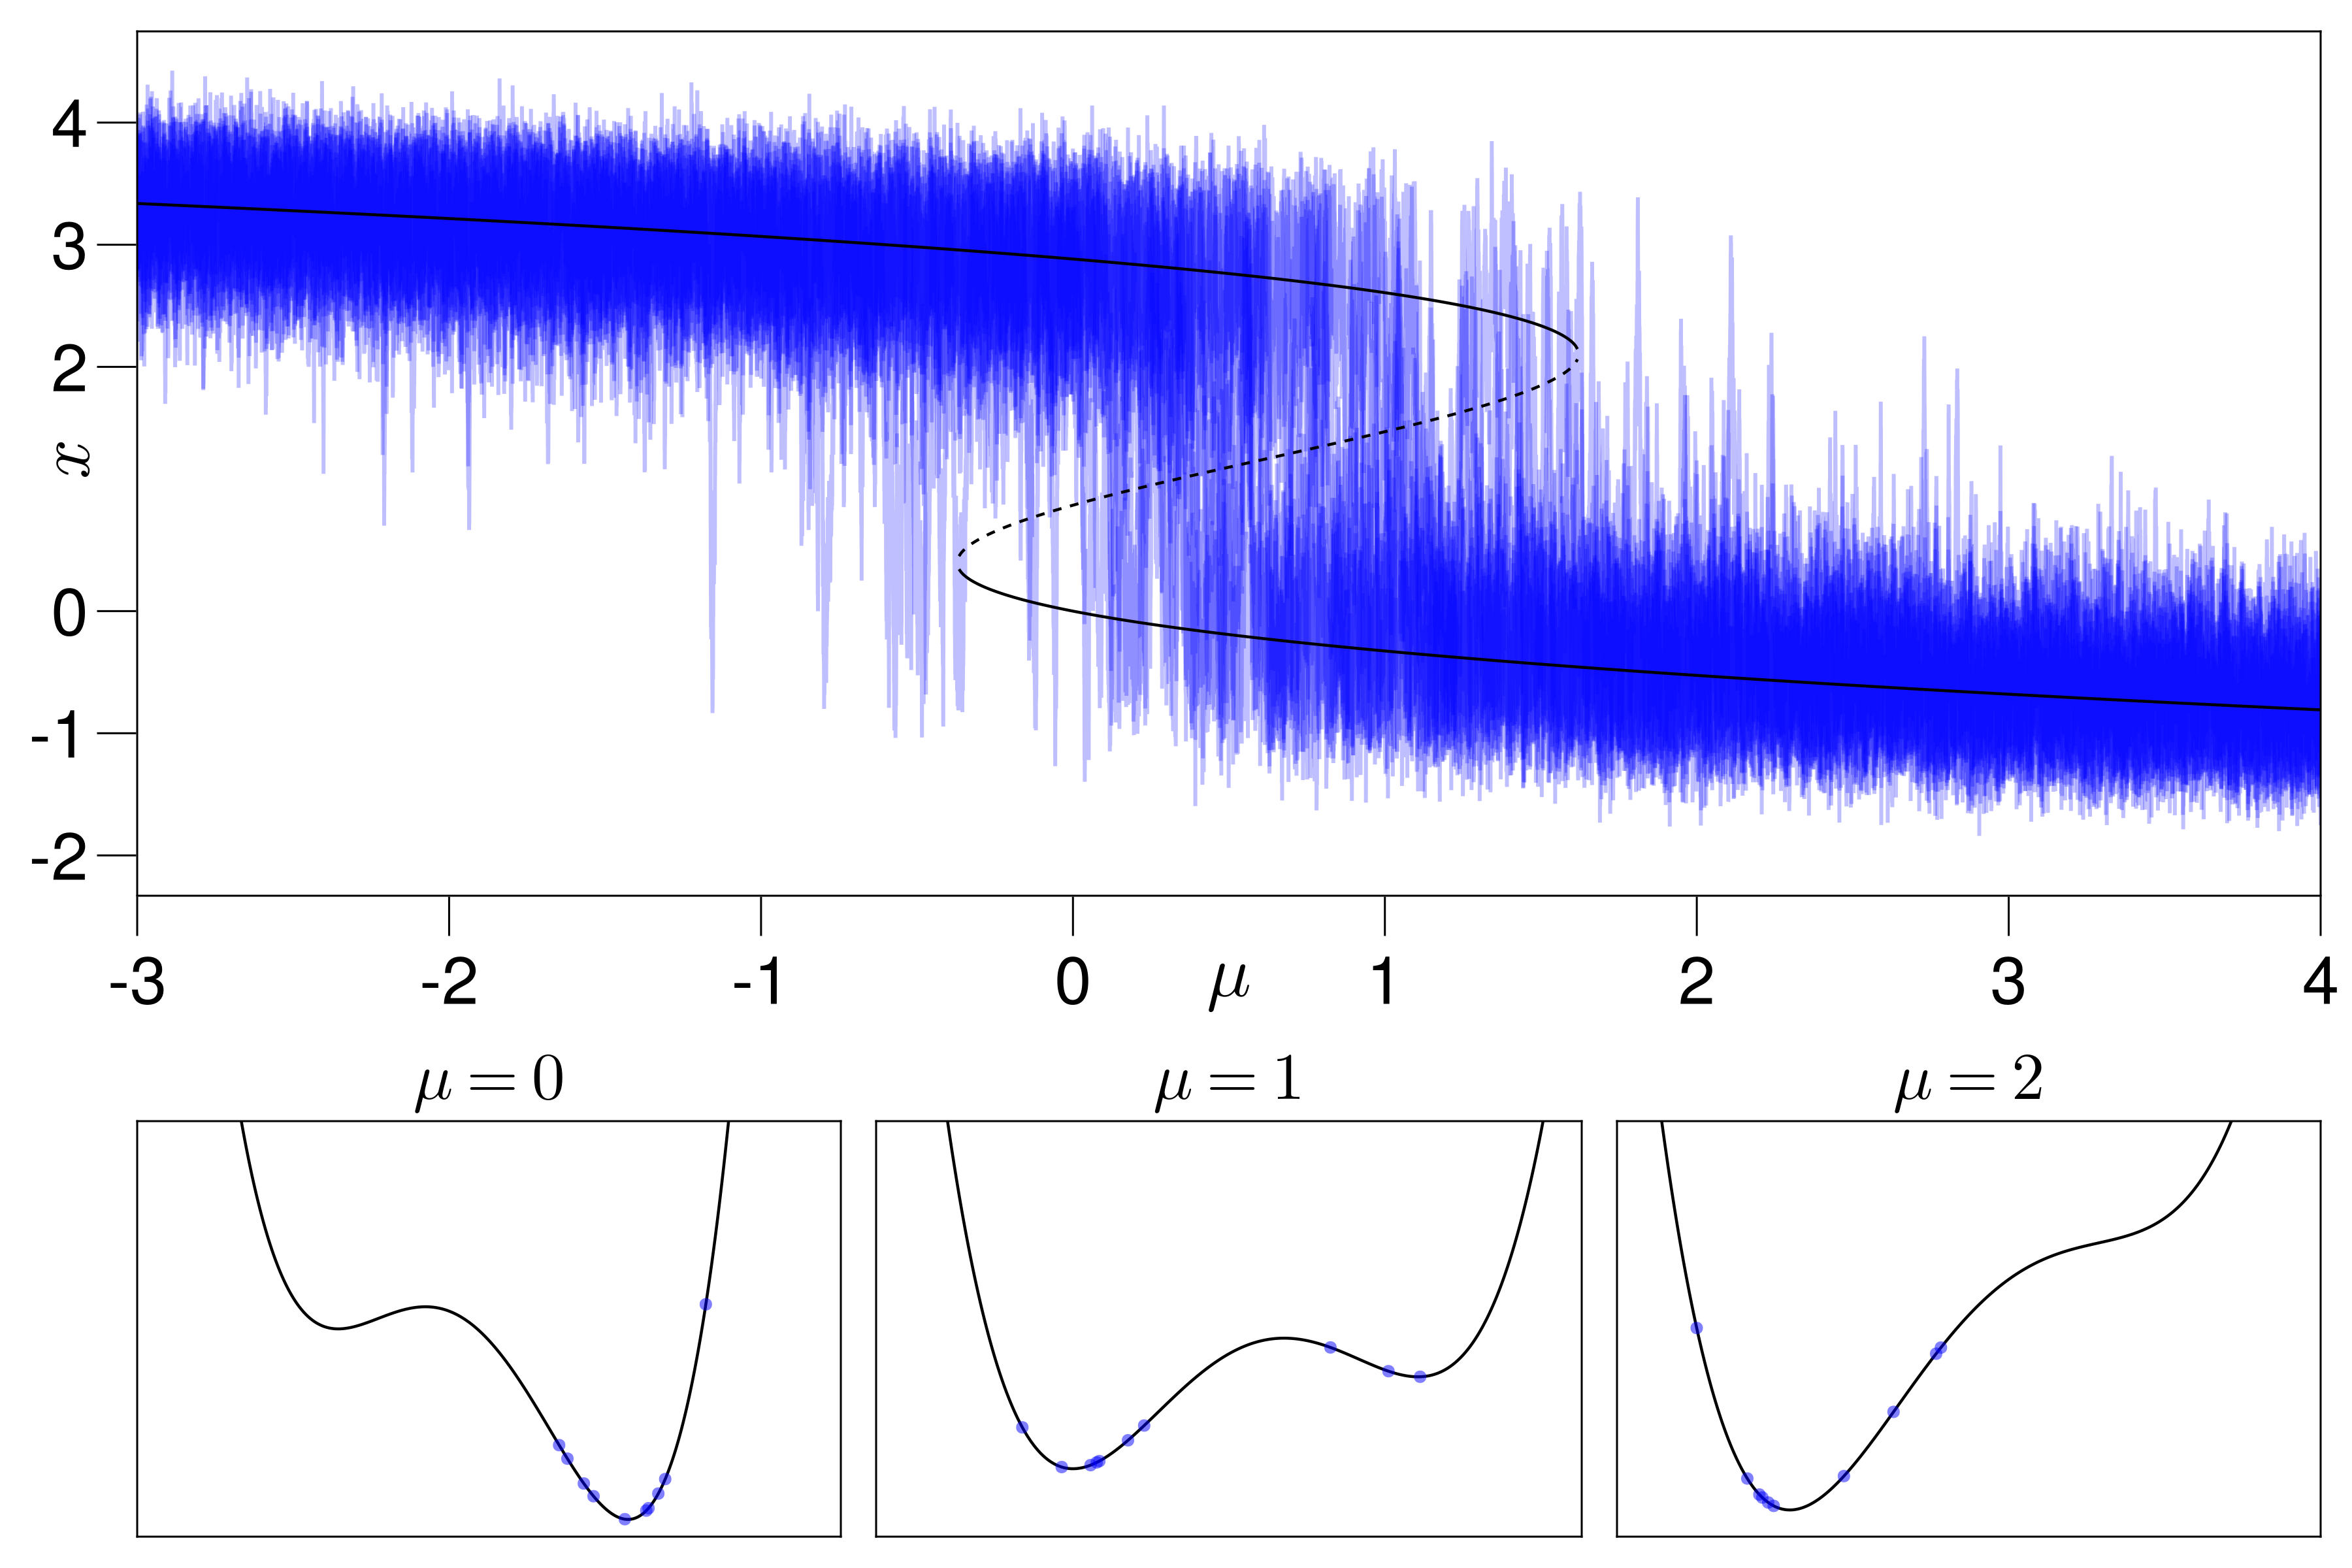
\includegraphics[keepaspectratio, width = \linewidth]{../figures/fig1.3.2.png}
        \caption{}
        \label{fig1.3.2}
   \end{subfigure}
    \caption{Ensemble sample paths of a bistable saddle-node bifurcation in low-noise (a) and highly stochastic (b) regimes. 
    The potential function is displayed in the bottom panels at parameter values $\mu=0,1$ in the bistability region and $\mu=2$ past the bifurcation; distribution of the ensemble states are plotted as dots on the potential function. 
We can clearly see how the high noise levels in (b) causes flickering anticipating substantially the critical threshold and this results in the ensemble states being considerably less clustered in the potential minima w.r.t. the low-noise case in (a). Details on the system and the potential function are provided in the Supplementary material.}
    \label{fig1.3}
\end{figure}
The newly introduced precursor, by its very nature, complicated the analysis of the dynamics far from the bifurcation since high level of noise may cause the system to switch back and forth between alternative stable states and, as previously established, the prediction of these noise-induced tipping is considerably harder than those that are associated to bifurcations. 
In 2012 the influence of \textit{strong noise} in a multi-decadal lake eutrophication experiment showed that skewness and autocorrelation display opposite trends w.r.t. the increase in variance \cite{Wang12} which led to the conclusion that the latter could have only be caused by flickering rather than CSD.
The meaningful consequence of this is that, in \textit{``highly stochastic dynamics"}, the switch to bistable regimes sets in quite earlier than CSD (see Figure \ref{fig1.3}), i.e. when the alternative attractor becomes strong enough such that the noise-induced fluctuations will cause excursions across the entire basin of attraction.
Further evidence of this was given one year later by Dakos, van Nes and Scheffer \cite{Dakos13} which systematically registered increase in variance and decrease of autocorrelation (symptomatic of flickering) in highly noisy but low-resolution timeseries well ahead of the CSD associated to a saddle-node bifurcation.
While all these results firmly placed skewness as an indicator of flickering, the increase in variance was now linked to both CSD and flickering depending on the noise-level embedded in the realizations of the stochastic process and the size shrinking of the basin of attraction in a multistable regime.
The underlying implication is that it would not always be possible to rely on timeseries data alone to distinguish between the two different drivers of critical transitions given the low dimensionality of the model, by which we mean that the mere observation of the temporal realizations of the stochastic processes will forcibly discard potentially useful information that could otherwise help to determine robustly the distance from upcoming thresholds.
As such, other works were starting to address the possibility of including spatial dependence in their models in the hope of enriching the forewarning capability of EWS.
\end{document}
